%\documentclass{article}
\documentclass[a4paper,12pt]{article}
\usepackage[12pt]{extsizes}
\usepackage[T2A]{fontenc}
\usepackage[utf8]{inputenc}
\usepackage[english, russian]{babel}
\usepackage[left=3cm,right=1.5cm,top=2cm,bottom=2cm]{geometry}
\usepackage{hyperref}
\usepackage{amssymb,amsmath,amsthm}
\usepackage{cleveref}
\usepackage{caption}
\usepackage{mathtools}
\usepackage{multirow}

\usepackage{subfig}  % или \usepackage{subcaption}
\usepackage{graphicx} % Required for inserting images
\usepackage{ulem}
\usepackage{amsmath}
\usepackage{geometry}
\geometry{top=2.5cm, bottom=2.5cm, left=2.5cm, right=2.5cm}
\usepackage{hyperref}
\usepackage{array}
\usepackage{booktabs}  % Для более красивых таблиц (по желанию)
\usepackage{tabularx}
\usepackage{enumitem}
\usepackage{titlesec}
\usepackage{appendix}
\usepackage{float}    % Для принудительной вставки картинок в определенное место (чтобы они не "плавали") [H]

\usepackage[nottoc,numbib]{tocbibind} % Пакет tocbibind добавляет в оглавление пункты, которые обычно туда не попадают: библиографию, список иллюстраций, список таблиц и т. д.

\begin{document}

% --------------------- Титульник ВКР СПбГУ -----------------------------
% Автор: Тоскин Николай, itonik@me.com
% Если заметили ошибку, напишите на email
% Если хотите добавить изменение самостоятельно:
% https://github.com/itonik/spbu_diploma/
% Использованы материалы:
% habr.com/ru/post/144648/
% cpsconf.ru
% Документы ниже могут уже быть неактуальны, тем не менее за годы ничего
% нового не появилось
% Текст:
% http://edu.spbu.ru/images/data/normativ_acts/local/20181030_10432_1.pdf
% Титульный лист:
% http://edu.spbu.ru/images/data/normativ_acts/local/20180703_6616_1.pdf
% -----------------------------------------------------------------------

% Титульный лист диплома СПбГУ
% Временное удаление foot на titlepage
\newgeometry{left=30mm, top=20mm, right=15mm, bottom=20mm, nohead, nofoot}
\begin{titlepage}
\begin{center}

\textbf{Санкт--Петербургский}
\textbf{государственный университет}

\vspace{35mm}

\textbf{\textit{\large Соловьев Дмитрий Николаевич}} \\[8mm]
% Название
\textbf{\large Выпускная квалификационная работа}\\[3mm]
\textbf{\textit{\large Система домашней автоматизации с использованием децентрализованного подхода в хранении и обработке данных.}}

\vspace{20mm}
Уровень образования: бакалавриат\\
Направление 02.03.02  «Фундаментальная информатика и информационные технологии»\\
Основная образовательная программа CB.5190.2021
«Большие данные и распределенная цифровая платформа»\\[25mm]
%Профиль «Исследование и проектирование систем управления\\ и обработки сигналов»\\[25mm]


% Научный руководитель, рецензент
\begin{flushright}
\begin{minipage}[t]{0.65\textwidth}
{Научный руководитель:} \\
доцент, кафедра компьютерного моделирования и \\многопроцессорных систем,\\к.ф.-м.н., PhD\\Корхов Владимир Владиславович

\vspace{10mm}

{Рецензент:} \\
доцент, кафедра компьютерного моделирования и \\многопроцессорных систем,\\к.т.н.\\Дик Геннадий Давидович
\end{minipage}
\end{flushright}

\vfill 

{Санкт-Петербург}
\par{\the\year{} г.}
\end{center}
\end{titlepage}
% Возвращаем настройки geometry обратно (то, что объявлено в преамбуле)
\restoregeometry
% Добавляем 1 к счетчику страниц ПОСЛЕ titlepage, чтобы исключить 
% влияние titlepage environment
\addtocounter{page}{1}



\section*{Аннотация}

С увеличением количества устройств интернет вещей (ИВ) в системах домашней автоматизации (СДА) остро встает вопрос топологий сетей, в которых находятся эти устройства, а также способах хранения и передачи данных между устройствами. Многим системам, использующим централизованный подход в хранении и обработке информации, свойственна существенная потеря функциональности при выходе из строя центрального узла. В ходе исследования были изучены принципы, методологии и архитектуры, применимые к программно-аппаратным комплексам для построения СДА и позволяющие повысить уровень безопасности данных, отказоустойчивость и увеличить скорость передачи информации в рамках системы за счет использования распределенного подхода к хранению и обработке информации, разработан прототип распределенной СДА. Результаты проведенного исследования и предложенная в нем архитектурная модель могут быть использованы не только в системах умных домов, но и в умных городах и на предприятиях.

\section*{Abstract}

With the increasing number of Internet of Things (IoT) devices in home automation systems (HAS), the topologies of the networks that house these devices, as well as how data is stored and transferred between devices, are becoming an issue. Many systems that use a centralized approach in storing and processing information are characterized by a significant loss of functionality when a central node fails. In the course of the research the principles, methodologies and architectures applicable to hardware-software complexes for the construction of ADS were studied, which allow to increase the level of data security, fault tolerance and increase the speed of information transfer within the system due to the use of distributed approach to information storage and processing, and a prototype of distributed ADS was developed. The results of the conducted research and the architectural model proposed in it can be used not only in smart home systems, but also in smart cities and enterprises.

\newpage

\tableofcontents

\newpage


\section{Введение}

\subsection{Актуальность темы}

Актуальность и практический аспект анализа систем и выбора оптимальной для построения системы домашней автоматизации:

\begin{enumerate}
    \item	Количество устройств с возможностью интеграции в систему умного дома среди потребителей быстро возрастает год к году. Особенности построения актуальных систем накладывает ограничения на масштабируемость системы, ее надежность и безопасность.
    \item	В системах домашней автоматизации с появлением новых типов устройств и попытки их интеграции возникают проблемы, связанные со скоростью реакции на события и с отсутствием приоритезации сообщений.
\end{enumerate}

\subsection{Объект исследования}
Объектом научно-исследовательской работы являются системы домашней автоматизации, системы хранения, передачи и обработки информации.

\subsection{Предмет исследования}
Предметом научно-исследовательской работы является оптимизация обработки и передачи данных между устройствами ИВ в системе домашней автоматизации.

\subsection{Постановка задачи}

В рамках данной работы ставится цель провести комплексное исследование существующих СДА на рынке, проанализировать применяемые в них протоколы и выявить основные недостатки. На основании этого выбрать оптимальный протокол и разработать прототип системы, отвечающий сформулированным требованиям и решающий обозначенный список проблем.

Для достижения этой цели были сформулированы начальные условия (требования):

\begin{enumerate}
    \item Сеть устройств в пределах одной зоны должна строиться по одноуровневому принципу, без централизованных узлов управления.
    \item Взаимодействие устройств внутри зоны осуществляется напрямую, без посредников (ЦУД).
    \item Для связи устройств из разных зон используются шлюзы-ретрансляторы, объединённые в единую распределённую сеть.
\end{enumerate}

Практическая значимость предлагаемого подхода:
\begin{itemize}
    \item Уменьшение задержек, расширение сфер применения: в предлагаемой системе уменьшается количество узлов между устройством-инициатором и устройством-актуатором (при нахождении в одной сети - до нуля), за счет чего увеличивается скорость выполнения команд и повышается общая отзывчивость системы, что расширяет сферы применения устройств ИВ для построения СДА, ранее нефункциональных ввиду относительно больших задержек.
    \item Повышение комфорта использования: данные о состоянии устройств, как и статистика, собираемая устройствами, хранится и обрабатывается на самих устройствах, что позволяет обеспечить короткое время восстановления работы после внештатных ситуаций (например, отключения питания) без длительной синхронизации.
    \item Упрощение настройки системы: благодаря использованию планировщика, автоматически распределяющего сценарии по устройствам, нет необходимости в ручной конфигурации каждого узла.
    \item Повышение отказоустойчивости: отказ сценария в одной локации возможен лишь при неисправности одного из двух устройств (инициатора и актуатора) и не зависит от иных устройств в сети. Объединение локаций, а также дистанционный мониторинг и управление системой осуществляется посредством распределенной системы шлюзов-ретрансляторов, что избавляет от единой точки отказа системы (точки входа).
    \item Повышение безопасности: распределенный подход для хранения сценариев и управления устройствами минимизирует получение злоумышленниками доступа ко всем устройствам. Система шлюзов-ретрансляторов, использующих VPN-соединение избавляет от единой точки отказа системы (точки входа).

\end{itemize}



\newpage

\section{Глава 1}

\subsection{Топологии беспроводных сетей}
Все перечисленные беспроводные сети работают в одном или нескольких вариантах
топологии. На рис.~\ref{fig:topologies} приведены топологии беспроводных сетей различных конфигураций.

\begin{figure}[h]
    \centering
    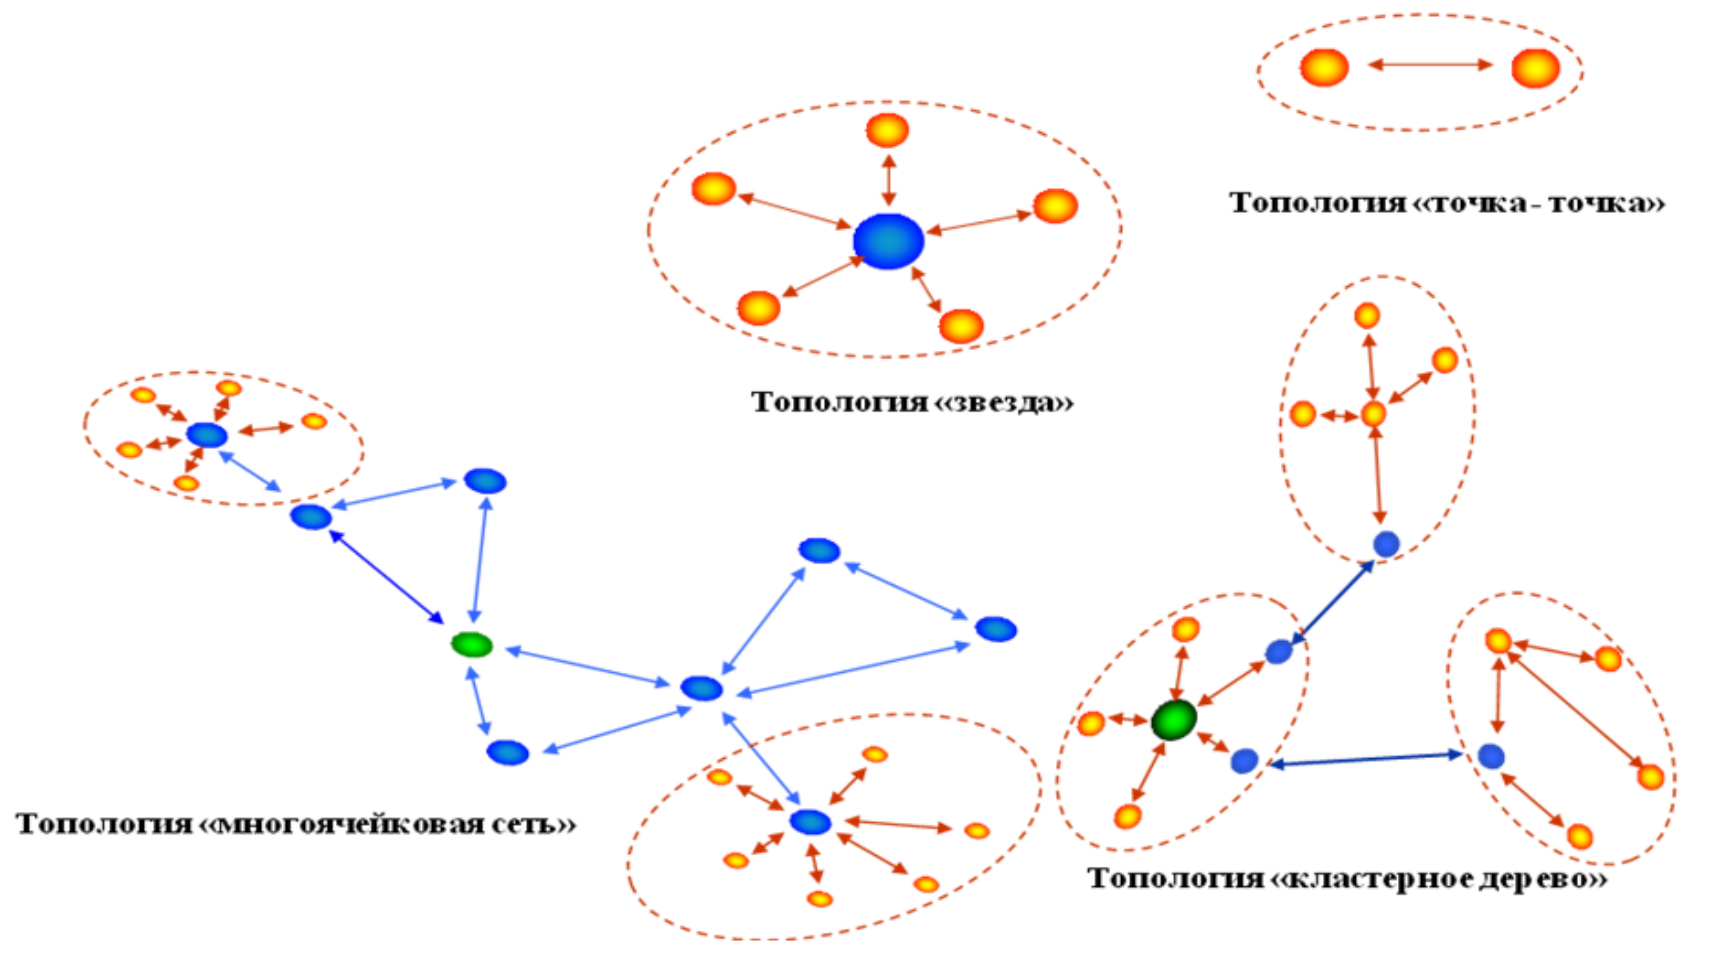
\includegraphics[width=0.8\textwidth]{images/Fig06.png}
    \caption{Топологии беспроводных сетей \cite{wirelessNetProtocols} }
    \label{fig:topologies}
\end{figure}



\subsubsection{Топология точка-точка}
Самый простой вариант организации сети из двух устройств. Как правило, узлы этой сети являются равноправными, то есть сеть одноранговая.
Эта топология характерна для Bluetooth, ANT, RFID, RuBee, PDC, WI-FI, Insteon, UWB, ZigBee и прочих.

\subsubsection{Топология «Звезда»}
Эта топология служит основой организации всех современных сетей связи и вычислительных сетей. Данную топологию используют протоколы WI-FI, Insteon, ZigBee, UWB, IDEN, CDMAOne, WIMAX, GSM, GPRS, UTMS.

\subsubsection{Ячеистая топология}
Ячеистая топология — базовая полносвязная топология компьютерных сетей и сетей связи, в которой каждая рабочая станция сети соединяется со всеми другими рабочими станциями этой же сети. Характеризуется высокой отказоустойчивостью, сложностью настройки и избыточным расходом кабеля в проводных сетях. Каждый узел имеет несколько возможных путей соединения с другими узлами, за счет этого такая топология очень устойчива. Так как исчезновение одного из каналов не приводит к потере соединения между двумя компьютерами. Эта топология допускает соединение большого количества узлов и характерна, как правило, для крупных сетей, она строится из полносвязной путем удаления некоторых возможных связей.
Топология применима для сетей с использованием протоколов UWB, WI-FI, Insteon, ZigBee, UWB, IDEN, CDMAOne, WIMAX, GSM, GPRS, UTMS.

\subsubsection{Топология «кластерное дерево»}
Топология «Кластерное дерево» образуется в основном в виде комбинаций вышеназванных топологий вычислительных сетей. Основание дерева вычислительной сети располагается в точке (корень), в которой собираются коммуникационные линии информации (ветви дерева).
Вычислительные сети с древовидной структурой строятся там, где невозможно непосредственное применение базовых сетевых структур в чистом виде.


\subsection{Протоколы беспроводных сетей}
В данный момент большинство производителей ИВ используют централизованный подход для построения СДА \cite{Rus_alternative}. В качестве центра умного дома (ЦУД) выступает устройство (хаб), объединяющее конечные устройства в единую сеть. Сценарии взаимодействия устройств могут быть локальными (сценарии хранятся в ЦУД) или облачными. Вариант с локальным расположением сценариев более предпочтительный, так как повышается отзывчивость системы и ее отказоустойчивость. Отдельную сложность представляет объединение устройств из разных экосистем: различные комбинации связей <<устройство>>, <<ЦУД>>, <<облако>>.
\begin{figure}[h]
    \centering
    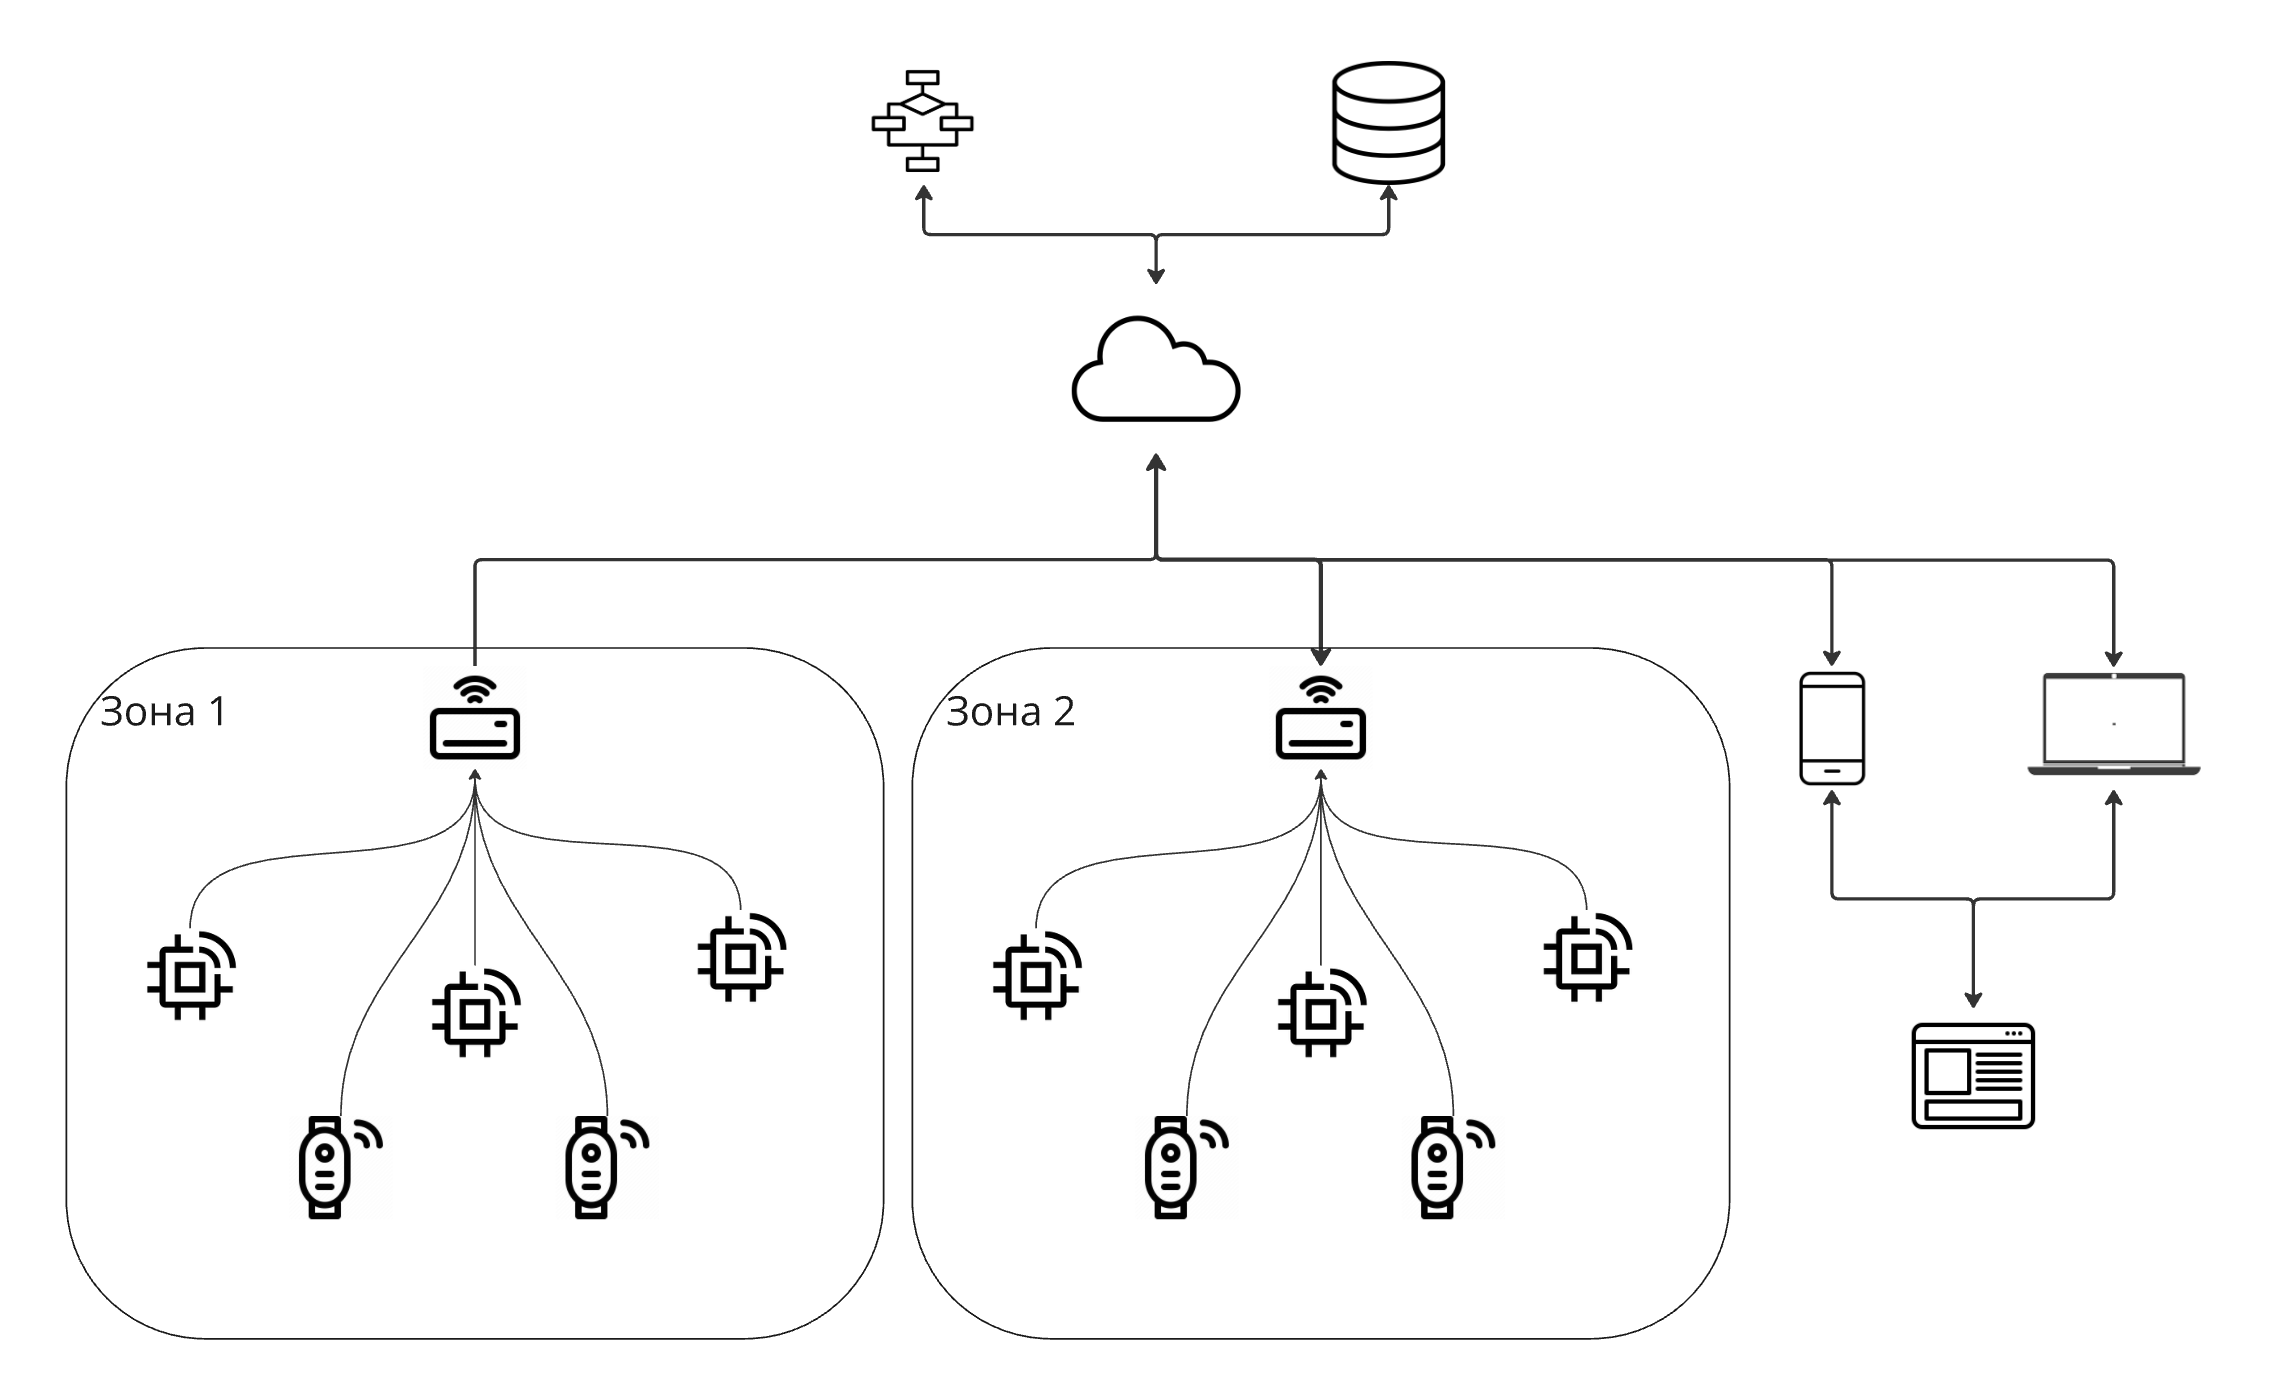
\includegraphics[width=0.8\textwidth]{images/CommertialAlternativeDesign.png}
    \caption{Пример СДА с облачной обработкой событий}
    \label{fig:cloud_event_processing}
\end{figure}

Большинство имеющихся на данный момент решений опираются на топологию <<дерево>>, где в качестве корня рассматривается ЦУД или облако, что проиллюстрированно на рис. \ref{fig:cloud_event_processing}. При этом структура может подразумевать наличие единственных ветвей из корня, например <<облако-ЦУД-устройства>> \cite{smart_home_review}. Тенденции 2023-2024 г. по переносу обработки событий в ЦУД, который ранее использовался лишь для маршрутизации сообщений от устройств к облаку, позволили увеличить надежность и уменьшить задержки в системе, но не исключили имеющиеся проблемы полностью.

Стоит различать аппаратные ограничения, не позволяющие изменить топологию системы, связанные с особенностью работы протокола, например, топологию Bluetooth, позволяющую организовывать только связи типа точка-точка или точка - множество устройств, и архитектуру системы УД, подразумевающую централизованное выполнение сценария в ЦУД либо облаке.






\subsubsection{Wi-Fi и Wi-Fi HaLow}

Протокол Wi-Fi относится к семейству стандартов IEEE 802.11, реализующих беспроводную передачу данных в различных частотных диапазонах:
\begin{itemize}
    \item 2{,}4 ГГц — стандарты 802.11b/g/n;
    \item 5 ГГц — 802.11a/ac;
    \item 6 ГГц — 802.11ax (Wi-Fi 6E).
\end{itemize}
Эти протоколы поддерживают высокую пропускную способность и широкое распространение благодаря простой интеграции в клиентские устройства. Однако они изначально не предназначены для энергоэффективных решений, что ограничивает их применение в системах домашней автоматизации, особенно если подразумевается использование батарейного питания. Так же различные виды конфигурации сети могут оказывать значительное влияние на время автономной работы IoT-устройства. \cite{WifiSmartHome}


\paragraph{IEEE 802.11ah (Wi-Fi HaLow)} — расширение Wi-Fi в суб-ГГц диапазоне для IoT и промышленных задач. Обеспечивает дальность до километра, поддержку до тысяч устройств и низкое энергопотребление, что проиллюстрированно на рис.  \ref{fig:wifi_energy_eff}, благодаря механизмам Target Wake Time и RAW. Сохраняет уровень MAC совместимым с Wi-Fi, унаследовав безопасность и QoS.

\begin{figure}[h]
    \centering
    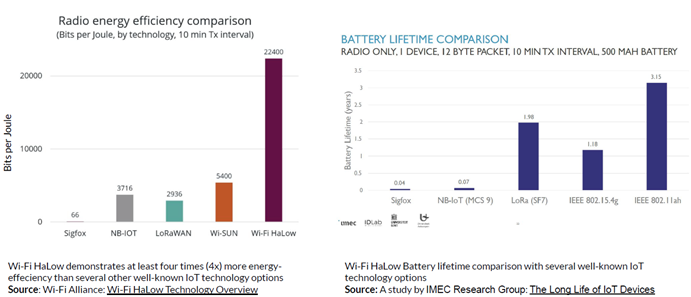
\includegraphics[width=0.8\textwidth]{images/WiFiEnergyEff.png}
    \caption{Сравнение энергоэффективности протоколов \cite{IMG_protocol_compare_power_eff}}
    \label{fig:wifi_energy_eff}
\end{figure}

\paragraph{Основные элементы архитектуры и топологии}
\begin{itemize}
  \item \textbf{Диапазон частот:} 863–928 МГц (региональные поддиапазоны).
  \item \textbf{Узлы:} 
    \begin{itemize}
      \item \emph{STA} (датчики/актуаторы) с поддержкой энергосбережения.
      \item \emph{AP} (Access Point), иногда \emph{Relay AP} (ретрансляторы).
    \end{itemize}
  \item \textbf{Топология:} нет встроенного mesh L2 -- дерево с ограниченной глубиной.
\end{itemize}

\paragraph{Преимущества и недостатки:}

в качестве преимуществ IEEE 802.11ah можно выделить большую дальность связи (до 3 км вне помещений при использовании ретранслятора Relay AP), высокую плотность подключений (возможность обслуживания сотен устройств одной точкой доступа), а также низкое энергопотребление при малой активности. Вместе с тем, стандарту присущи: низкая пропускная способность по сравнению с Wi-Fi в диапазонах 2,4/5/6 ГГц, более высокая сложность и стоимость модулей по сравнению с устройствами на базе 802.15.4, из-за чего данный протокол не получил широкого распространения среди потребительских устройств, заняв только небольшую нишу промышленных IoT-устройств; а также сложности лицензирования различных диапазонов частот для разных стран.



\subsubsection{Bluetooth Low Energy (BLE) и Bluetooth Mesh}
Т.к. BLE Mesh лишь расширение стандарта, использующий особым образом режим рекламы для лавинообразного передачи сообщений, по техническим характеристикам он сильно похож на BLE. Для поддержания совместимости было использовано лавинообразное рассылка (flooding \cite{BLE_mesh_spec}), которая с большим количеством устройств может значительно увеличить территорию покрытия, но, с другой стороны, может привести к избыточной загруженности каналов, что после некоторой отметки в количестве устройств может привести к потерям пакетов. Так же метод является неоптимальным при небольшом количестве устройств ввиду счетчика TTL который на каждом шаге уменьшается и может обнулиться, не дойдя до адресата [20].

\subsubsection{Zigbee}
Протокол, основанный на IEEE 802.15.4, описывающий построение беспроводной персональной сети. Спецификация Zigbee ориентирована на приложения, требующие гарантированной безопасной передачи данных при относительно небольших скоростях и возможности длительной работы сетевых устройств от автономных источников питания (батарей). Основная особенность технологии Zigbee заключается в том, что она при малом энергопотреблении поддерживает не только простые топологии сети («точка-точка», «дерево» и «звезда»), но и самоорганизующуюся и самовосстанавливающуюся ячеистую (mesh) топологию с ретрансляцией и маршрутизацией сообщений. Кроме того, спецификация Zigbee содержит возможность выбора алгоритма маршрутизации в зависимости от требований приложения и состояния сети.
Основными областями применения технологии Zigbee являются беспроводные сенсорные сети, автоматизация жилья («Умный дом» и «Интеллектуальное здание»), медицинское оборудование, системы промышленного мониторинга и управления, а также бытовая электроника и «периферия» персональных компьютеров.
Способность к самоорганизации и самовосстановлению, ячеистая (mesh-) топология, защищённость, высокая помехоустойчивость, низкое энергопотребление и отсутствие необходимости получения частотного разрешения делают Zigbee-сеть подходящей основой для беспроводной инфраструктуры систем позиционирования в режиме реального времени (RTLS).
В России, как и в большинстве стран мира за исключением США, ЕС и Австралии разрешенная частота составляет 2.4 ГГц, которая является общей для других технологий, таких как WiFi и Bluetooth, что может привести к избыточной загруженности каналов и большой потере сообщений.

\subsubsection{Сравнение представленных протоколов}
Был составлен сравнительный график различных протоколов передачи сообщений.\

\begin{figure}[h]
    \centering
    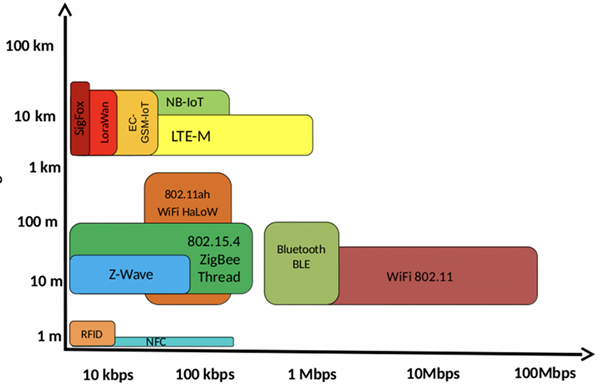
\includegraphics[width=0.8\textwidth]{images/Fig07.png}
    \captionsetup{justification=centering}
    \caption{Сравнение беспроводных протоколов передачи данных по дальности и скорости передачи. \cite{IMG_protocol_compare} }
    \label{fig:protocols_range_vs_speed}
\end{figure}

Так же была составлена сравнительная таблица.
Wi-Fi Mesh (IEEE 802.11s) и BLE Mesh работают полностью без единого сетевого координатора: в Wi-Fi Mesh каждый узел (Mesh Point) самостоятельно участвует в маршрутизации
по протоколу HWMP, а BLE Mesh применяет управляемое наводнение без роли координатора доставки. Zigbee же требует наличия PAN Coordinator’а, который создаёт и управляет
сетью, выдавая адреса устройствам-роутерам. Z-Wave полагается на Primary Controller (и Static Update Controller) для добавления узлов и хранения
топологии, без которого сама сеть не синхронизируется. Thread формально выбирает «лидера», но все Router-узлы равноправны: нет жёсткого единственного
координатора, а маршруты поддерживаются децентрализованно через MLE-сообщения. При этом большинство протоколов (Wi-Fi Mesh, BLE Mesh, Zigbee, Thread) работают в перенаселённой
полосе 2.4 GHz – зона 2.4 GHz страдает высоким уровнем помех и зашумлённостью каналов, тогда как Z-Wave (868/915 MHz) избегает этой проблемы.

Для построения распределенной самовосстанавливающейся сети без единой точки отказа и с наименьшей задержкой, лучше выбирать Wi-Fi Mesh или BLE Mesh, хотя они не лишены
компромисов: нуждаются в широкой полосе и часто сталкиваются с помехами на частоте 2.4ГГц. Для снижения влияния радио-шумов 2.4ГГц и повышения надёжности на больших
расстояниях предпочтительнее Z-Wave на суб-ГГц, пусть и с центральным контроллером.

\begin{table}[h!]
    \centering
    \renewcommand{\arraystretch}{1.3}
    \begin{tabularx}{\textwidth}{|l|X|X|X|X|}
        \hline
        \textbf{Имя} & \textbf{Пропускная способность} & \textbf{Дальность} & \textbf{Энергопотребление} & \textbf{Протокол маршрутизации} \\
        \hline
        WiFi Mesh & до 1,300 Мбит/с & до 100 м в помещении и до 300 м на открытом пространстве & от нескольких мВт до нескольких сотен мВт & HWMP с возможностью изменения \\
        \hline
        BLE Mesh & до 125 Кбит/с & до 100 м в помещении и до 300 м на открытой местности & от нескольких мкВт до нескольких мВт & Flooding \\
        \hline
        Z-wave & до 100 Кбит/с & до 100 м в помещении и до 300 м на открытой местности & от нескольких мкВт до нескольких мВт & Закрытый протокол \\
        \hline
        Zigbee & от 20 до 250 Кбит/с & от 10 до 100 м в помещении и до 400 м на открытом пространстве & от нескольких мкВт до нескольких мВт & AODV с возможностью изменения \\
        \hline
    \end{tabularx}
    \caption{Сравнение беспроводных mesh-технологий}
\end{table}

\subsubsection{Доступность для разработчиков платформ, поддерживающих представленные протоколы}

В среде Arduino IDE наиболее зрелая поддержка реализована для плат серии ESP32 DevKitC на базе модуля ESP-WROOM-32: доступен API для построения Wi-Fi Mesh,
однако готовых примеров в составе «arduino-esp32» нет, а поддержка BLE Mesh на уровне Arduino отсутствует, требуя прямой работы с ESP-IDF. Платы ESP32-C6 и
ESP32-H2 оснащены аппаратным радио IEEE 802.15.4 (Zigbee/Thread), но в текущих версиях core для Arduino-ESP32 их поддержка нестабильна и не включает
демонстрационных примеров; для полноценной работы требуется использовать свежие ветки «arduino-esp32» или компилировать примеры из ESP-IDF.

Со стороны STMicroelectronics наиболее популярна плата P-NUCLEO-WB55RG (Nucleo-WB55RG) на базе STM32WB55, где через STM32duino core и библиотеку STM32duinoBLE
доступны примеры по BLE, но для Thread и Zigbee необходимо обращаться к STM32CubeWB SDK и демонстрациям на сайте производителя. Аналогично, плата STM32W-RFCKIT
поддерживается лишь в рамках STM32CubeWB и не имеет официальных Arduino-библиотек или готовых sketch’ей.

\newpage

\section{Глава 2}

\subsection{Краткое описание предлагаемой системы}
Централизованные СДА, имеющие ЦУД, обладая несомненными преимуществами, такими как простота настройки и реализации,
также имеют ряд недостатков: низкая скорость реакции, невысокая надежность и безопасность, сильно зависящая от ЦУД
и облачной инфраструктуры. Для интеграции устройств, находящихся в разных сетях, используется централизованная
координация через единое облако. На рис.~\ref{fig:GlobalSystemDesing} представлена архитектура предлагаемой гибридной системы, подразумевающей
прямое взаимодействие устройств в СДА.


\begin{figure}[h]
    \centering
    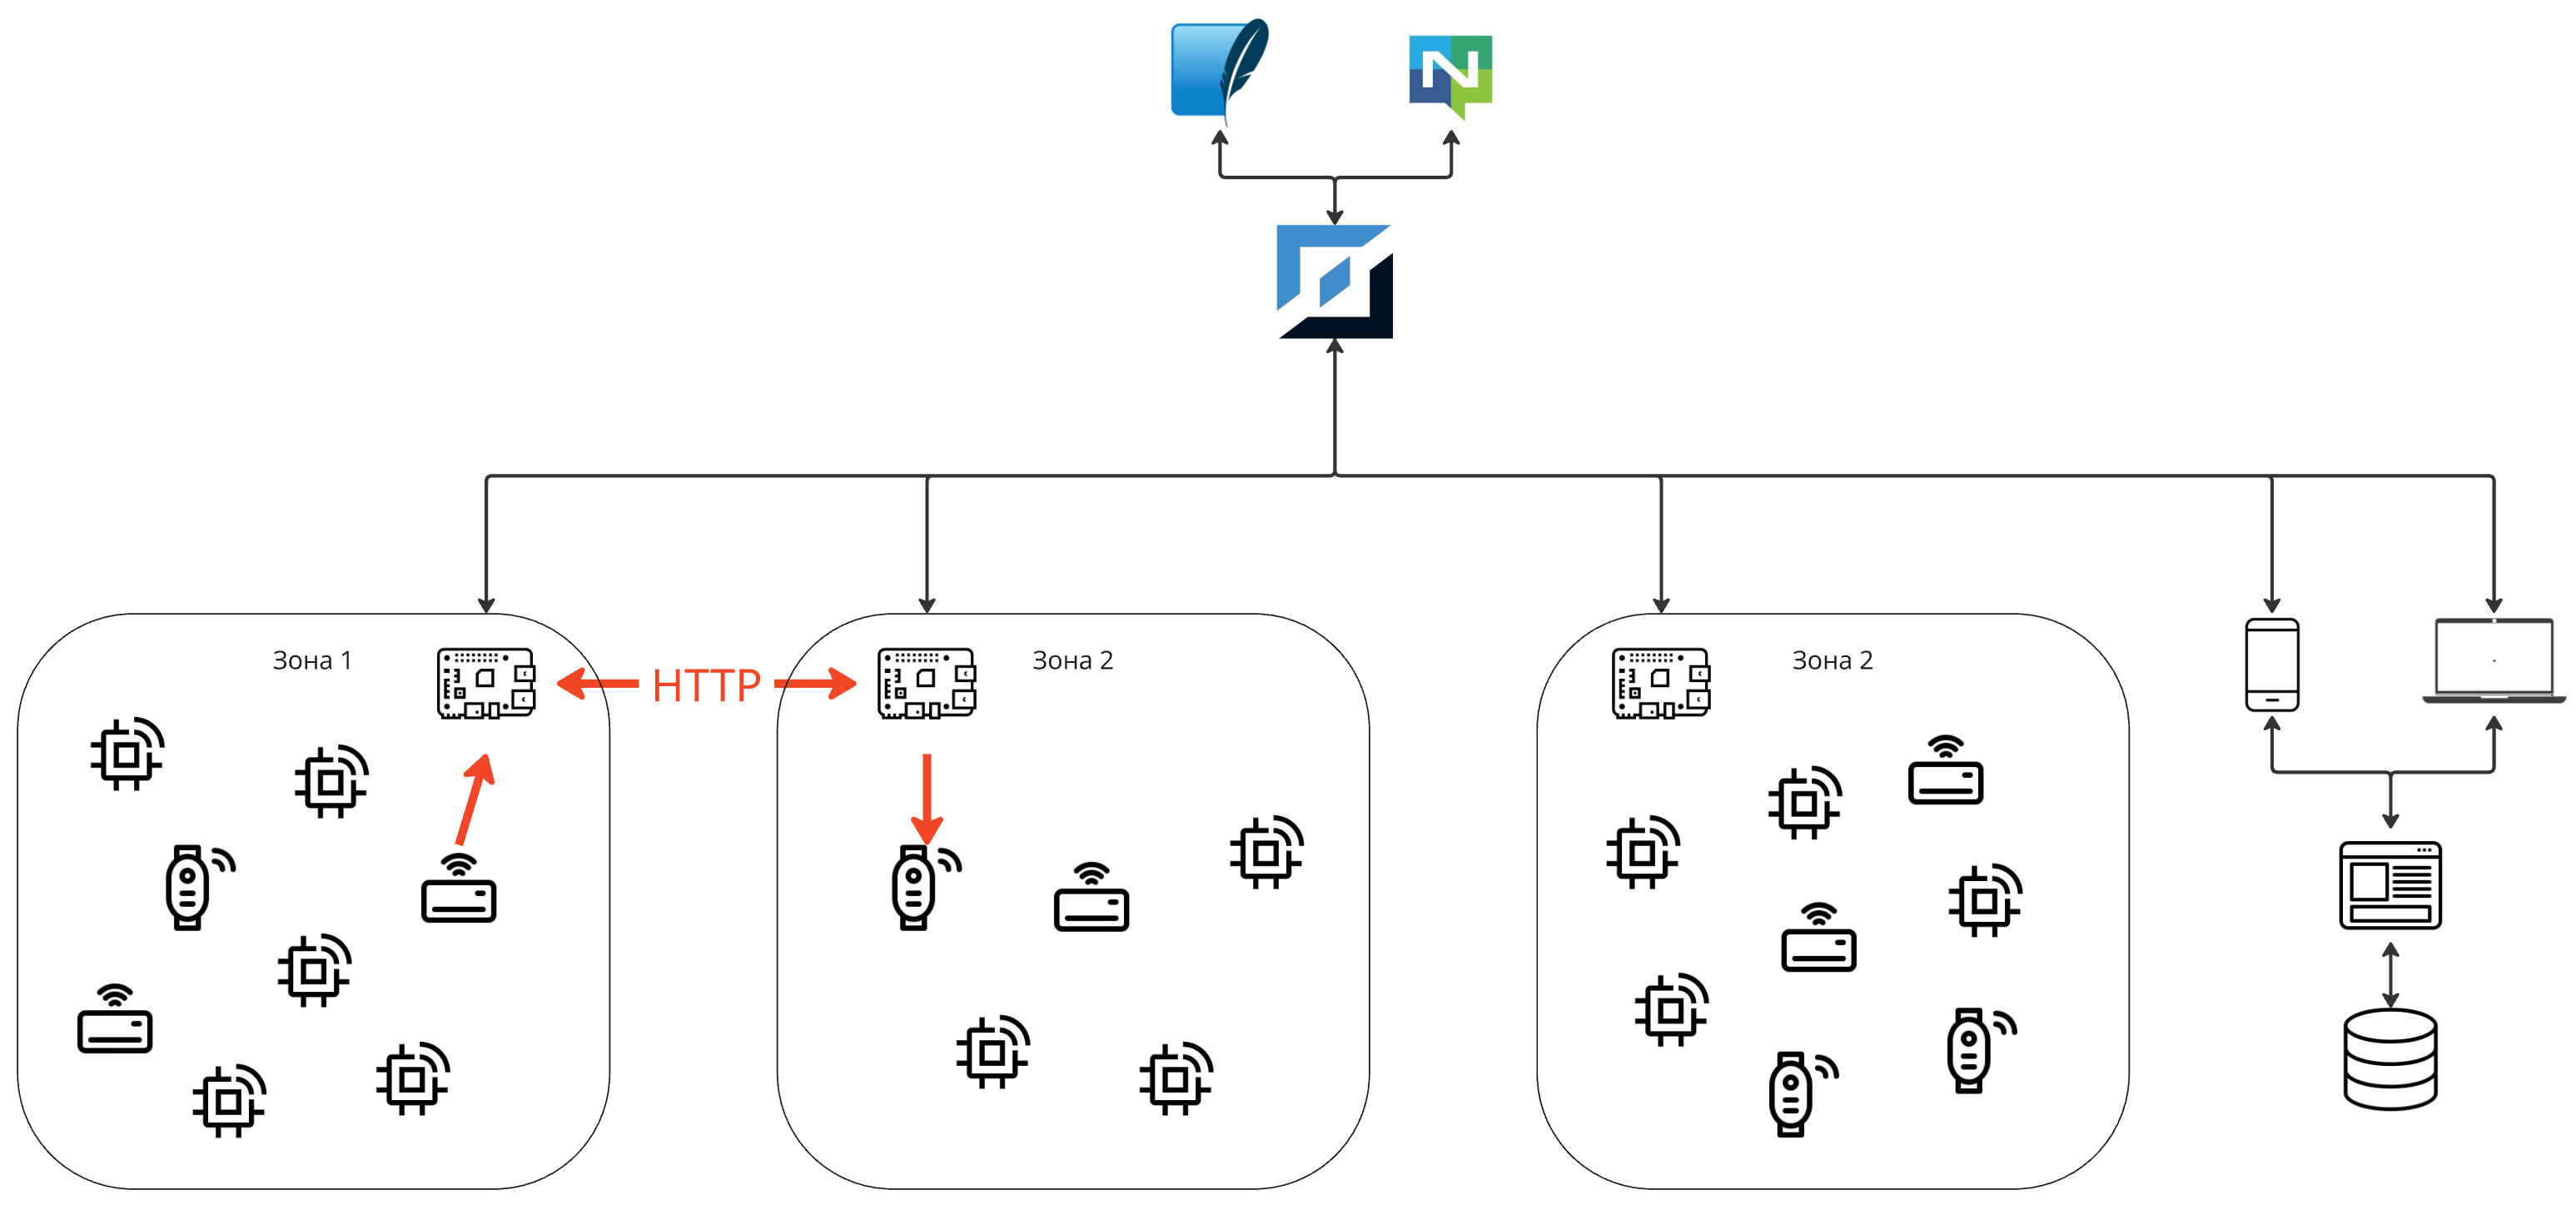
\includegraphics[width=0.8\textwidth]{images/GlobalSystemDesing.png}
    \caption{Пример СДА с распределенной структурой}
    \label{fig:GlobalSystemDesing}
\end{figure}

Для взаимодействия физически разнесенных устройств предлагается использование
шлюзов-ретрансляторов, которые выполняют функцию объединения зон в единую сеть,
распределяют по устройствам обновленную конфигурацию сети, а также предоставляют функцию управления умным домом извне.
Предложенная система уменьшает количество промежуточных узлов между устройством, порождающим событие, и устройством
исполнителем (при нахождении устройств в одной зоне до нуля). Данное решение кроме повышения надежности системы также
уменьшает задержку передачи информации, повышает отказоустойчивость системы и ее безопасность \cite{SecuritySmartHome, SecuritySmartHome2}.

\begin{figure}[H]
    \centering
    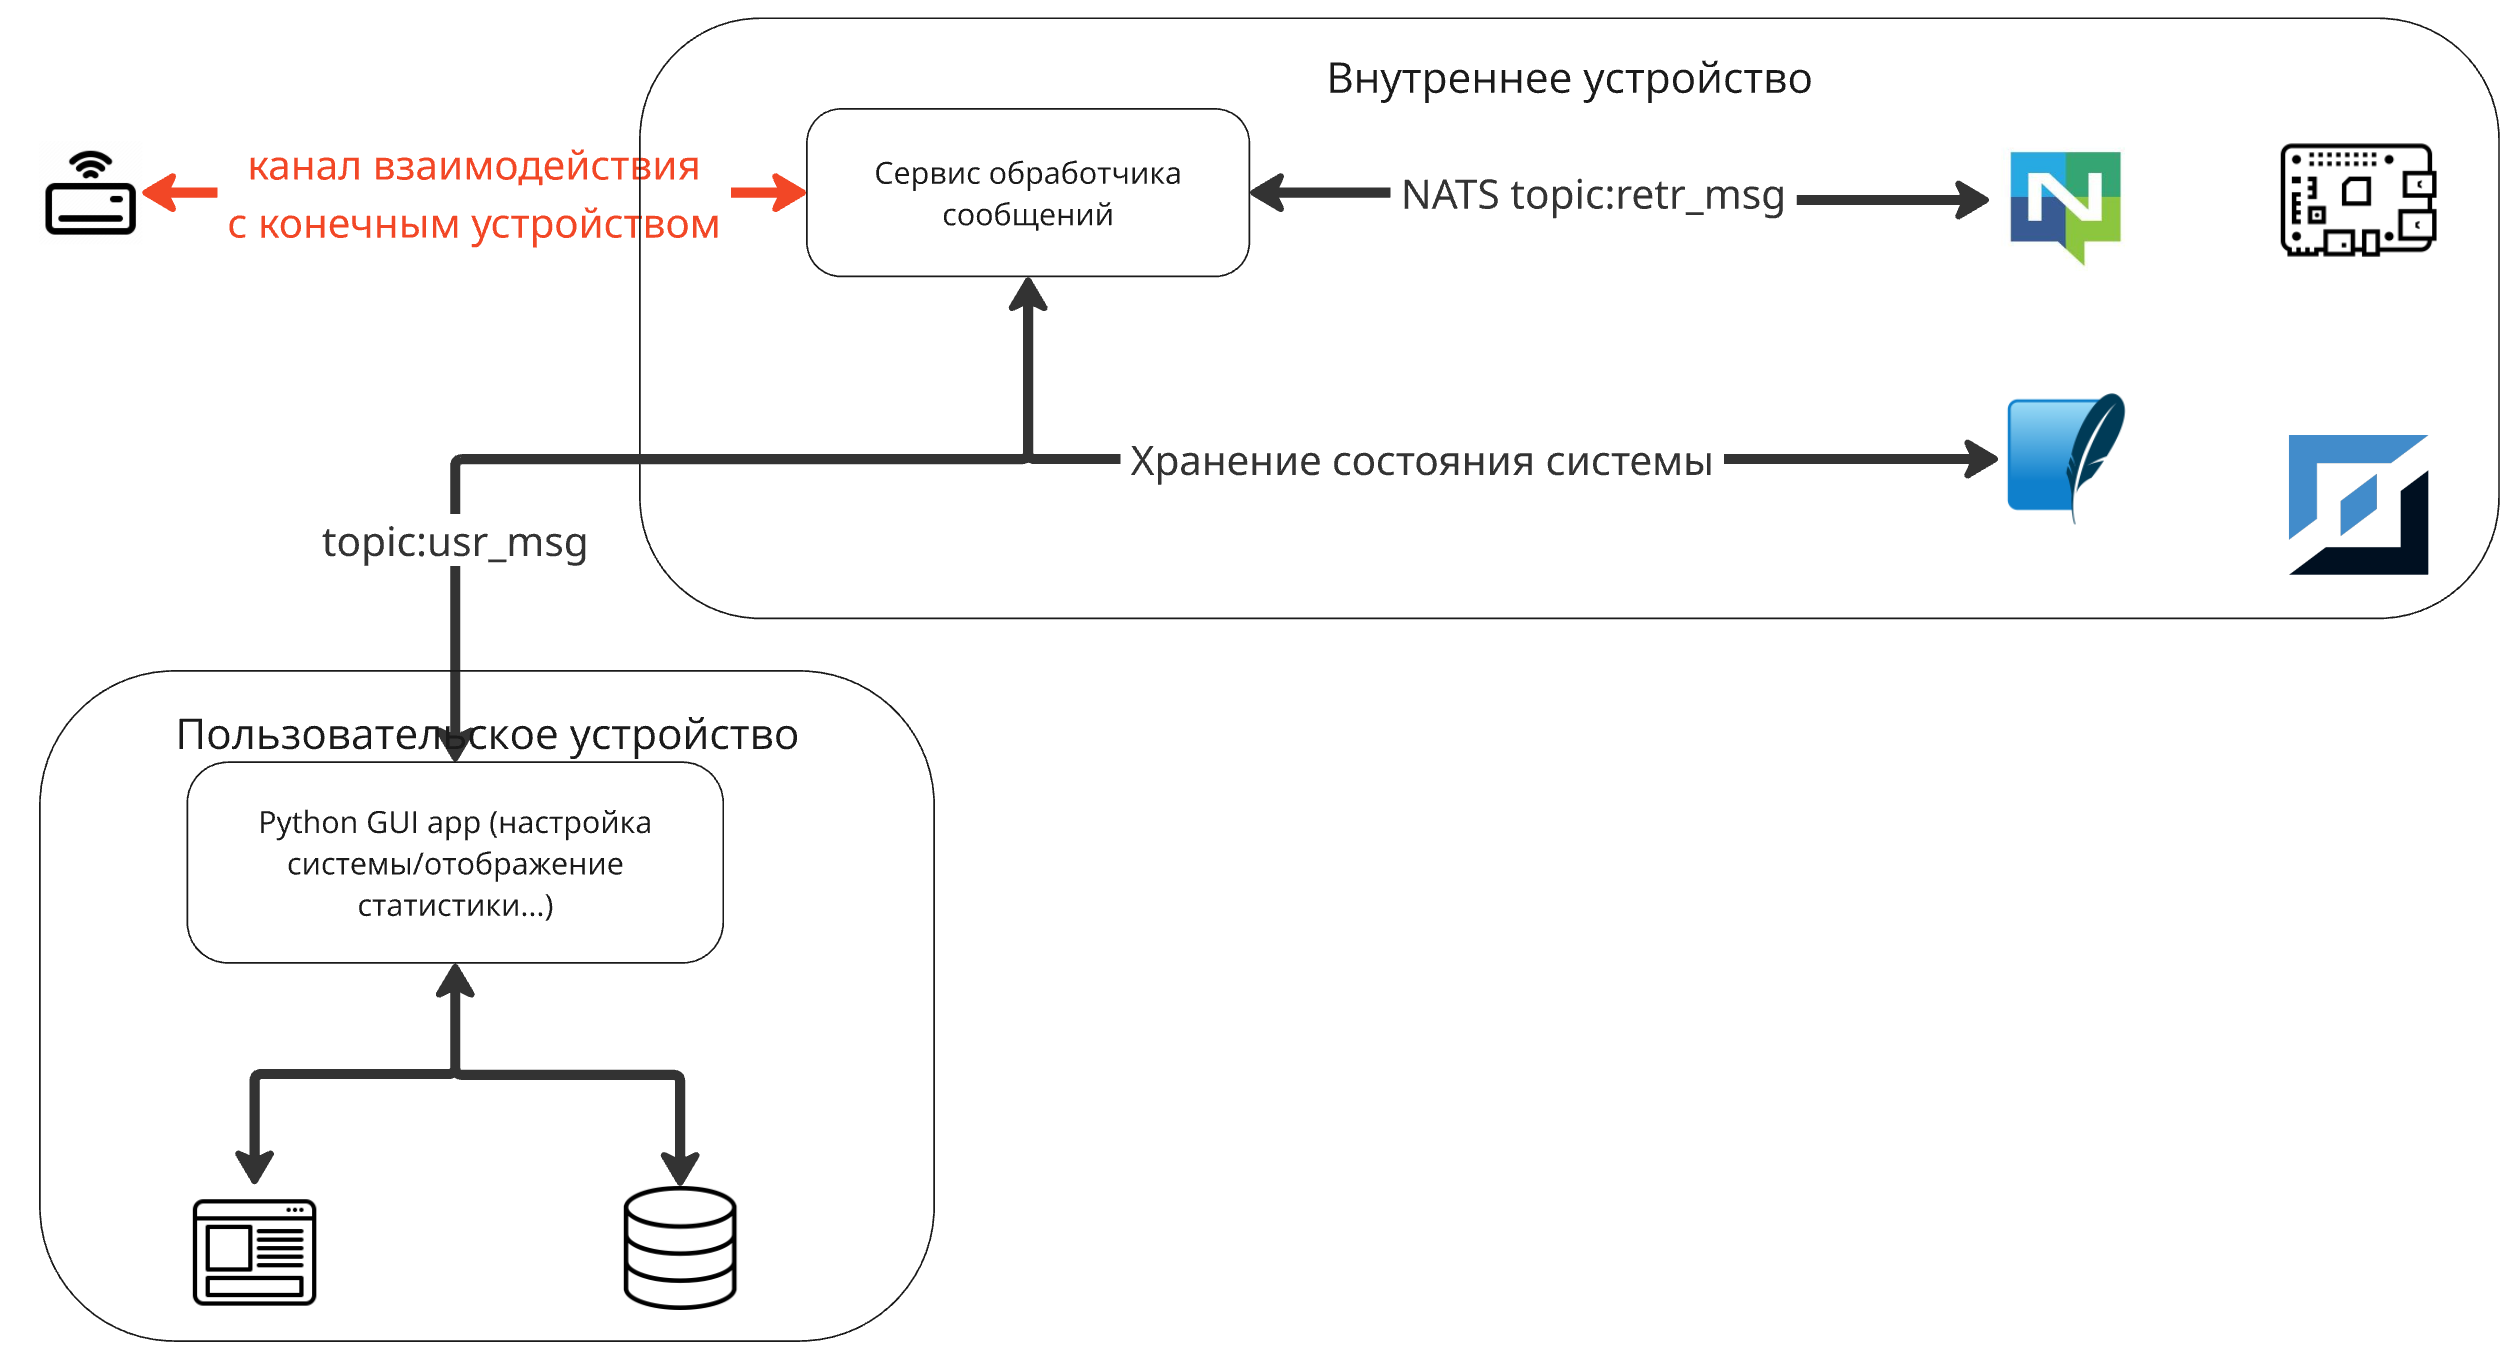
\includegraphics[width=0.8\textwidth]{images/InternalSystemDesign.png}
    \captionsetup{justification=centering}
    \caption{Компонентная структура и процессы взаимодействия в\\кластере K0s предложеннной системы}
    \label{fig:InternalSystemDesign}
\end{figure}


Шлюзы-ретрансляторы -- кластер K0s -- при выходе из строя какого-то узла, например, зоны
K, перестанут обрабатываться межзонные события, связанные с зоной К. При этом функционал внутри и вне зоны
К не изменится.

\begin{figure}[H]
    \centering
    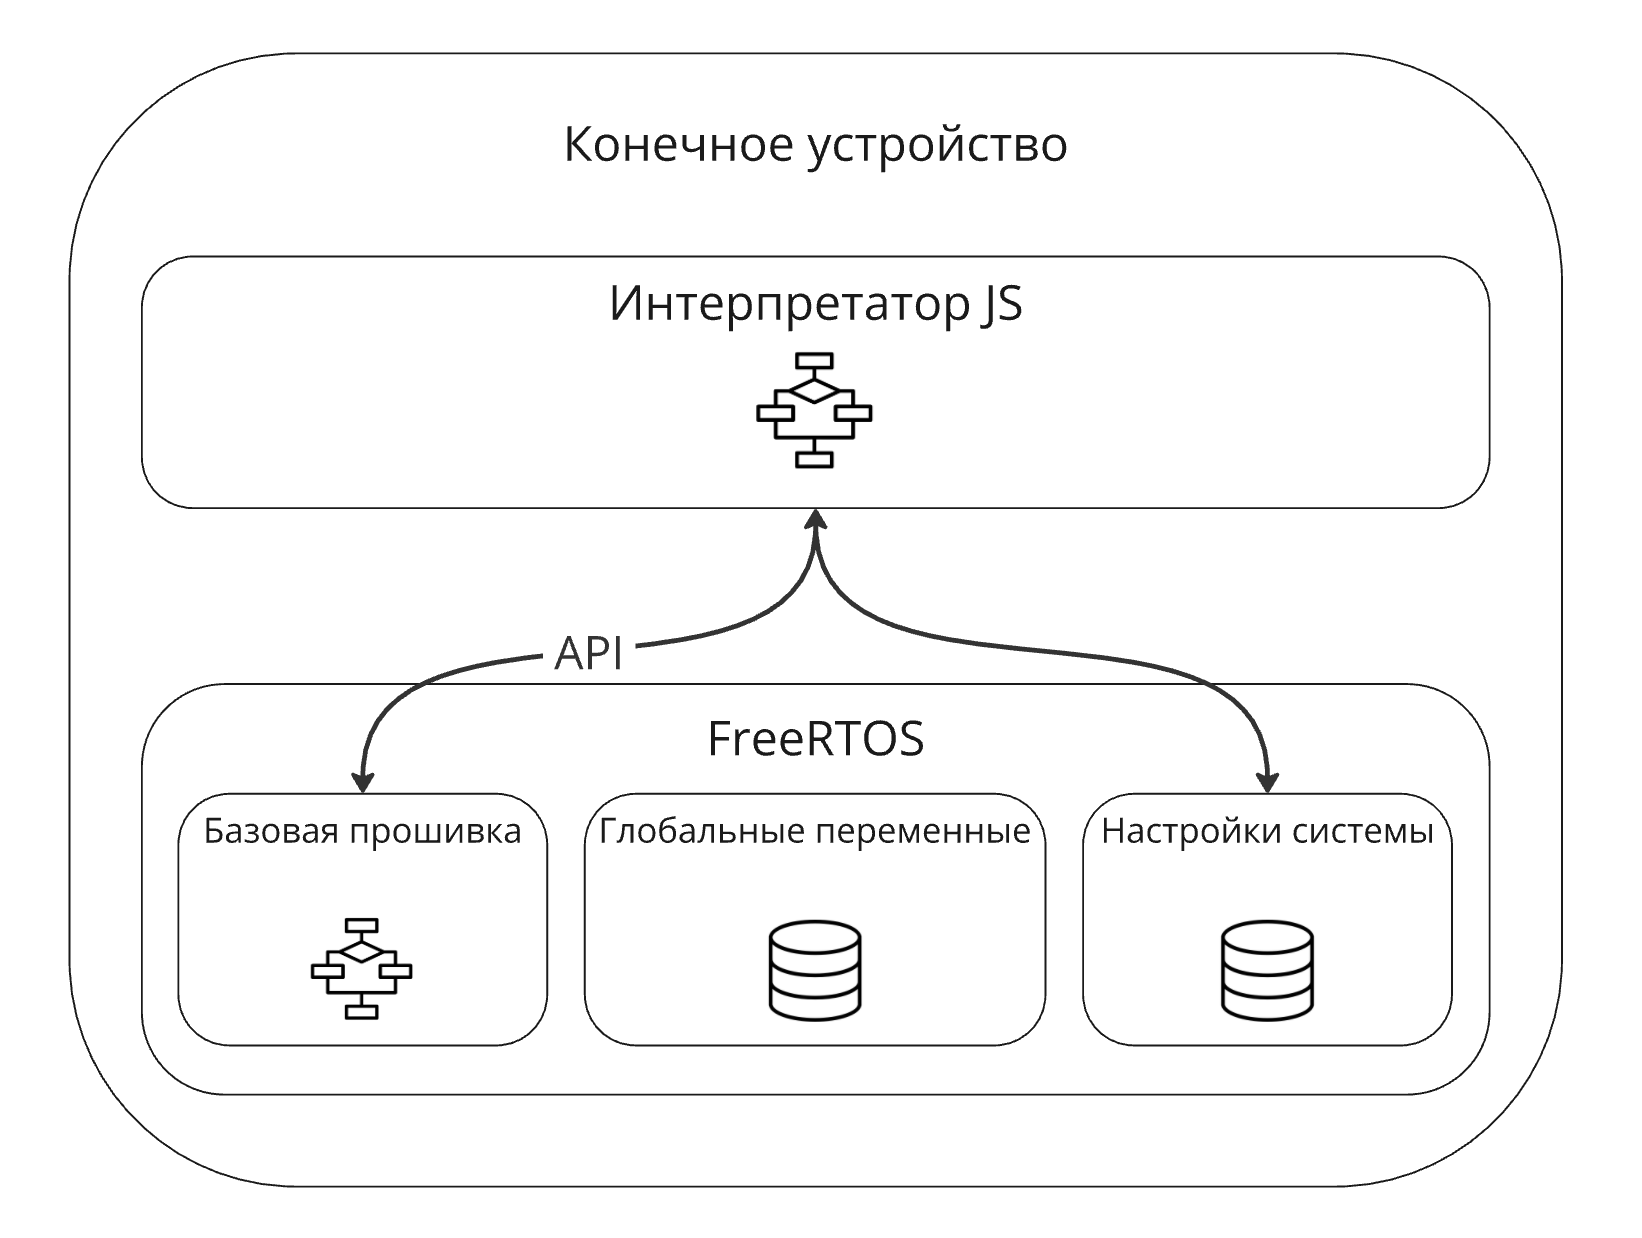
\includegraphics[width=0.8\textwidth]{images/Fig05.png}
    \caption{Реализация конечного устройства}
    \label{fig:end_device}
\end{figure}

Програмная часть каждого конечного устройства представляет из себя двухуровневую систему, как показано на рис.~\ref{fig:end_device}:
низкоуровневую прошивку, написанную с использованем FreeRTOS и предоставляющую API для высокоуровневой части для
управления, и высокоуровневую прошивку, написанную на языке JavaScript и запускающуюся посредством интерпретатора на
конечном устройстве. JS часть может быть легко изменена извне через настройку системы. Такой подход
позволяет вынести логику взаимодействия из ЦУД в конечные устройства и передавать данные напрямую и сразу локально
исполнять сценарии. Во время прототипирования были использованы различные протоколы передачи информации, в итоге
были использованы наиболее гибкие в настройке радиомодули SI4432.

\subsection{Выбранная топология системы}
Для передачи сообщений между конечными устройствами описываемая СДА использует радиомодули, взаимодействующие между собой посредством широковещательной передачи (broadcast), при которой каждое сообщение может быть принято любым узлом в зоне радиодоступа. Сигнал принимают все модули, но обрабатывают его лишь те, чей фильтр (например, по адресу или типу пакета) его пропускает. С точки зрения классических сетевых определений, говорить о чёткой топологии здесь затруднительно: физического соединения между узлами нет, а сама передача осуществляется через общую радиосреду. Такая структура ближе всего к логической топологии типа "шина" (bus), поскольку сигнал распространяется по общему каналу связи и доступен всем участникам сети. Однако корректнее описывать такую организацию как сеть с разделяемой средой доступа (shared medium) и логикой point-to-multipoint, где один узел может потенциально вещать всем, но приём зависит от контекста.

\subsection{Взаимодействие устройств}
Для связи устройств в рамках сети предлагается использование протокола для обмена сообщений по шаблону «наблюдатель» (Observer). В котором каждое устройство сверяет полученное сообщение со списком реакций на оповещения, и, если оповещение есть в списке, запускает выполнение команды. Наглядно демонстацию отличий Observer от Pub-Sub можно увидеть на рис.~\ref{fig:Observer_vs_pub_sub}.

\begin{figure}[h]
    \centering
    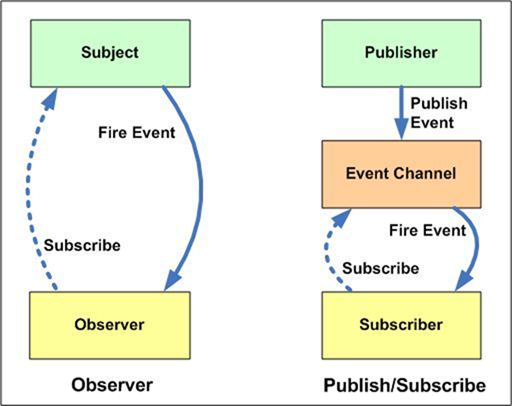
\includegraphics[width=0.6\textwidth]{images/Fig08.png}
    \caption{Отличие observer от Publisher-Subscriber \cite{IMG_observer_vs_pub_sub}}
    \label{fig:Observer_vs_pub_sub}
\end{figure}

\subsection{Добавление устройств и настройка сценариев}

Система домашней автоматизации состоит из конечных устройств, связанных по радиоканалу, и шлюзов-ретрансляторов, представляющих собой одноплатные компьютеры с установленными сервисами \texttt{k0s}. Настройка системы выполняется через единое графическое приложение, содержащее кнопку для начала настройки, поле для изменения параметров и кнопку для применения изменений.

\begin{enumerate}[label=\textbf{\arabic*.}]
    \item \textbf{Перевод системы в режим настройки.} 
    
    Пользователь нажимает кнопку <<Начать настройку системы>> в графическом интерфейсе. Приложение отправляет управляющую команду на все шлюзы-ретрансляторы, которые, в свою очередь, передают её конечным устройствам. Устройства переходят из режима эксплуатации в режим настройки и готовы к приёму новой конфигурации.
    
    \item \textbf{Внесение и отправка изменений.} 
    
    Через предоставленное текстовое или графическое поле в приложении вносятся необходимые изменения конфигурации. Это могут быть новые сценарии взаимодействия, логика работы исполнительных устройств и параметры ретрансляции сообщений. После завершения редактирования пользователь нажимает кнопку <<Применить настройки>>, и новая конфигурация передаётся на шлюзы-ретрансляторы.
    
    \item \textbf{Распространение конфигурации на конечные устройства.} 
    
    Шлюзы-ретрансляторы получают обновлённую конфигурацию и передают её по радиоканалу на исполнительные устройства. Датчики не требуют настройки, так как они только передают сообщения. Исполнительные устройства анализируют входящие сигналы и запускают соответствующие действия по заданным сценариям. После успешного применения настроек система может быть переведена обратно в режим работы тем же интерфейсом.
\end{enumerate}





\subsection{Обработка событий}
Каждое устройство-исполнитель хранит набор сценариев. Сценарии связаны с событиями. При выполнении события устройство сверяет события-активаторы, соответствующие сценариям, и, если события совпали, начинает выполнение соответствующего сценария. Сценарии представляют собой фрагменты кода JS, интерпретируемые на конечных устройствах. Их передача осуществляется в виде текстового формата JSON. Происходит их поэтапное выполнение.

\begin{figure}[h]
    \centering
    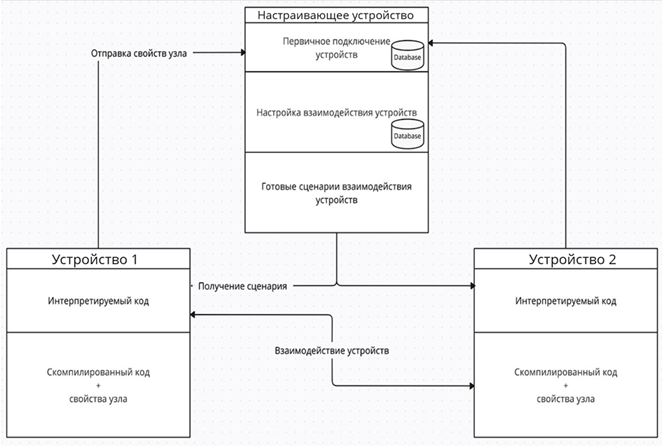
\includegraphics[width=0.8\textwidth]{images/Fig09.png}
    \caption{Пример взаимодействий конечных устройств}
    \label{fig:Connect_end_device_example}
\end{figure}


\newpage

\section{Глава 3}

\subsection{Графический интерфейс}
Был написано графическое приложение рис.~\ref{fig:GUI_base} на языке Python c использованием фреймворка Qt, в котором производилась настройка системы и ее отладка.

\begin{figure}[H]
    \centering
    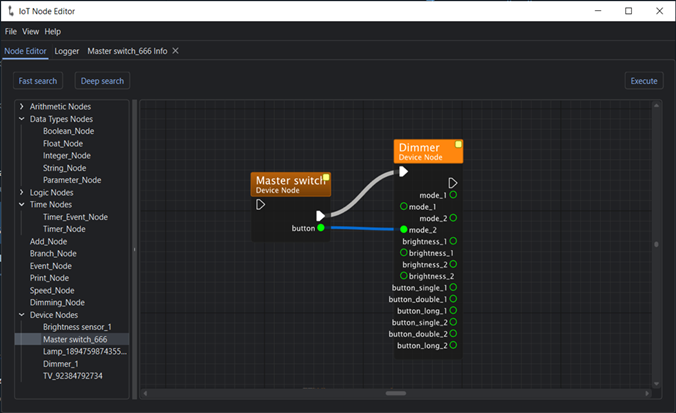
\includegraphics[width=0.8\textwidth]{images/Fig11.png}
    \captionsetup{justification=centering}
    \caption{Графическое приложение с созданным внутри\\сценарием для конечных устройств}
    \label{fig:GUI_base}
\end{figure}

Графический интерфейс позволяет прописывать и более сложные сценарии взадимодействия устройств, что можно увидеть на рис.~\ref{fig:GUI_adv}

\begin{figure}[H]
    \centering
    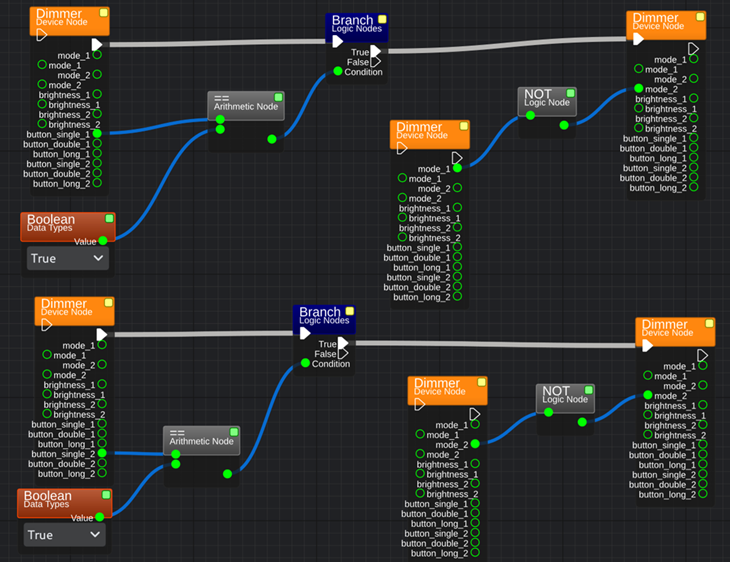
\includegraphics[width=0.8\textwidth]{images/Fig12.png}
    \caption{Пример более сложного сценария взаимодействия устройств}
    \label{fig:GUI_adv}
\end{figure}

\subsection{Планировщик}
Было опробовано два варианта распределения сценариев: их хранение и исполнение на устройстве-отправителе, порождающем событие и хранение сценариев на устройстве-исполнителе. В рамках проведенных экспериментов было установлено, что некоторые сложные команды, последовательный набор действий для первого варианта проводят к значительному увеличению времени обработки и излишней загруженности радиоканала, что потенциально уменьшает максимальное число устройств в системе.
Планировщик осуществляет преобразование визуальных узлов и связей в JS код, выполняя синтаксический анализ, преобразованием узлов в лексемы с последующем объединением их в единый исполняемый файл. Так же в задачи планировщика входит разбиение файла настроек на компоненты связанности и определение целевого устройства, на которое будет отправлен сценарий.
Также для дальнейшего тестирования система была сконфигурирована для работы с использованием ЦУД и для распределенной работы.

\newpage

\section{Глава 4}
\subsection{Тестирование и полученные оценки}
Для корректности тестирования и сравнимости подходов, ввиду отличия протоколов передачи данных, использования разных
микроконтроллеров в существующих системах и иных отличий, исходная система была переконфигурирована для работы как с
ЦУД, так и без ЦУД. Таким образом, проведя замеры задержек от возникновения события до реакции, можно оценить численно
преимущество предложенной архитектуры. В таблице приведены результаты замеров на каждом этапе: время передачи
пакета сообщения, время обработки события для каждой системы, что позволило использовать эти данные без привязки к
конкретной реализации. Были проведены замеры времени задержек выполнения программы на микроконтроллере STM32F411
(25МГц), выступавшим в качестве конечного устройства, и одноплатным компьютером Raspberry pi 3b+. Тестирование
одноплатного компьютера проводилось на системе Raspberry Pi OS 19.11, базирующейся на Debian 12. Использовался GCC 15
с опциями: <<-mcpu=native, -O2>>. При тестировании микроконтроллеров использовалась STM32duino FreeRTOS v10.3.2 с
библиотекой RadioLib v7.1.2. Радиомодули, представленные SI4432, использовались со стандартными параметрами.

\begin{table}[h!]
    \centering
    \begin{tabular}{|>{\centering\arraybackslash}p{1cm}|>{\centering\arraybackslash}p{8cm}|>{\centering\arraybackslash}p{2.5cm}|}
    \hline
    \textbf{п/п} & \textbf{Тип операции} & \textbf{Время операции} \\
    \hline
    1 & Передача в рамках одной зоны & 197 мс \\
    \hline
    2 & Выполнение 1 примитива интерпретатора на микроконтроллере & 18 мс \\
    \hline
    3 & Выполнение 1 примитива интерпретатора на одноплатном компьютере & 0{,}24 мс \\
    \hline
    4 & Общая задержка системы при использовании ЦУД & 407 мс \\
    \hline
    5 & Общая задержка системы без использования ЦУД & 231 мс \\
    \hline
    6 & Задержка СУД <<Умный дом с Алисой>> от Яндекс & $\sim$470 мс \\
    \hline
    \end{tabular}
    \caption{Среднее время выполнения операций}
\end{table}
    


Использовалось готовое решение на базе протокола Zigbee с ЦУД в виде YNDX-00510 \cite{YNDX_hub} и
лампой YNDX-00558. Лучшим способом сокращения задержек в СУД является уменьшение задержек в передаче
информации.Предложенный выше подход позволяет почти в вдвое сократить задержку (в рамках тестирования спроектированной
СУД) и более чем втрое по сравнению с представленными на рынке решениями.

\subsection{Вывод}
Предложен подход к построению распределенной системы домашней автоматизации, проведено сравнение с решением,
представленным на рынке. В дальнейшем предполагается исследовать возможные
уязвимости данной системы, построить и протестировать прототип распределенной системы с использованием шлюзов-ретрансляторов,
объединенных в единую сеть посретсвом VPN.

\newpage
\begin{thebibliography}{40}
\bibitem{wirelessNetProtocols} Колыбельников~А.\:И. Обзор технологий беспроводных сетей // ТРУДЫ МФТИ. 2012. Т.~4. №~2 С.~3--29.
\bibitem{Rus_alternative} Шерчков~А.\:В. Анализ существующих технических решений <<Умный дом>> // Молодежный вестник Уфимского государственного авиационного технического университета. 2020. №~1 С.~153--155.
\bibitem{WifiSmartHome} Montori~F., Contigiani~R., Bedogni~L., Is WiFi suitable for energy efficient IoT deployments? A performance study // 2017 IEEE 3rd International Forum on Research and Technologies for Society and Industry (RTSI). 2017. pp. 1-5, doi: 10.1109/RTSI.2017.8065943.
\bibitem{smart_home_review} Тукмачева~Ю.\:А. Обзор и анализ автоматизированных систем <<Умный дом>>, представленных на российском сегменте рынка // Вестник науки. 2022. Т.~4. №~10 С.~139--144.
\bibitem{SecuritySmartHome} Некрасов~П.\:В., Жариков~А.\:М., Козин~Д.\:А. Обеспечение безопасности беспроводных каналов связи киберфизических систем типа «Умный дом» // Безопасность информационных технологий. 2024. Т.~31. №~1 С.~54--62.
\bibitem{SecuritySmartHome2} Vardakis~G., Hatzivasilis~G., Koutsaki~E., Papadakis~N. Review of smart-home security using the internet of things // Electronics. 2024. No~13 P.~33--43.
\bibitem{YNDX_hub} Центр умного дома «Яндекс Хаб» модель YNDX-00510. Инструкция по эксплуатации [Электронный ресурс]: \url{URL: https://yastatic.net/s3/doc-binary/src/support/smart-home/hub/hub-manual.pdf} (дата обращения: 17.03.2025).
\bibitem{BLE_mesh_spec} Specifications and Documents Mesh Protocol [Электронный ресурс]: \url{URL: https://www.bluetooth.com/specifications/specs/html/?src=MshPRT_v1.1/out/en/index-en.html} (дата обращения: 11.05.2025).
\bibitem{IMG_protocol_compare} Сравнительный анализ стандартов связи для сетей IoT [Электронный ресурс]: \url{URL: https://habr.com/ru/companies/msw/articles/720518/} (дата обращения: 11.05.2025).

\bibitem{IMG_protocol_compare_power_eff} Wi-Fi HaLow™ and LoRaWAN: How do the technologies compare? [Электронный ресурс]: \url{URL: https://dev.wi-fi.org/zh-hans/beacon/y-zachary-freeman/wi-fi-halow-and-lorawan-how-do-the-technologies-compare} (дата обращения: 11.05.2025).

\bibitem{IMG_observer_vs_pub_sub} Observer vs Pub-Sub [Электронный ресурс]: \url{URL: https://habr.com/ru/articles/270339/} (дата обращения: 11.05.2025).

\end{thebibliography}

\newpage
\appendix
\renewcommand{\thesection}{\Alph{section}} % Нумерация буквами A, B, C…

% Заголовок первого приложения
\section*{Приложение A. Исходные коды и дополнительные материалы}
\addcontentsline{toc}{section}{Приложение A. Исходные коды и дополнительные материалы}

\begin{enumerate}[label=\arabic*.]
  \item Solovjev D. Distributed smart home cluster  [Электронный ресурс]: 
        \url{URL: https://github.com/Dmitrij-Solovjev/distributed-smart-home-cluster}
        (дата обращения: 11.05.2025). \\
        \emph{Примечание:} Кластер на базе K0s с сервисами для ретрансляции сообщений и общей настройки системы.
        
  \item Solovjev D. IoT Base Device [Электронный ресурс]: 
        \url{URL: https://github.com/Dmitrij-Solovjev/IoT-Base-Device} 
        (дата обращения: 11.05.2025). \\
        \emph{Примечание:} Прошивка для микроконтроллера на FreeRTOS, реализующая логику домашней автоматизации.
\end{enumerate}


\end{document}